\documentclass[10pt, a4paper]{beamer}
\usepackage{graphics}
\usetheme{Berkeley}
\usecolortheme{sidebartab}
\usepackage{array}
\begin{document}
    \setbeamertemplate{sidebar left}{}
    \title{Progress Presentation-I}
    \subtitle{e-Yantra Summer Intership-2016 \\ FreeRTOS on LPC2148}
    \author{K V S Sumakar\\Kartikeyan V\\
    Mentor:\\ Rutuja\\Deepa }
    \institute{IIT Bombay}
    \date{\today}
    %\addtobeamertemplate{sidebar left}{}{\includegraphics[scale = 0.3]{logowithtext.png}}
    \frame{\titlepage}

\setbeamertemplate{sidebar left}[sidebar theme]
\section{Overview of Project}
\begin{frame}{Overview of Project}
    
    \begin{itemize}
        \item Project Name : FreeRTOS on LPC2148
        \item Objective : To create modules on the implementation of basic FreeRTOS concepts on LPC2148
        \item Deliverables : Documentation of each and every FreeRTOS concepts that has been implemented on LPC2148.
    \end{itemize}
\end{frame}

\section{Overview of Task}
\begin{frame}{Overview of Task}
    
\begin{center}
\begin{tabular}{ | m{.5cm} | m{5cm}| m{2cm} | } 
\hline
Sr No. & TASKS & DEADLINES \\ 
\hline
1. & Basics of RTOS  & 4 days  \\ 
\hline
2.& Multi-Tasking Examples & 5 days\\ 
\hline
3. & Concepts of Semaphore and Mutex examples based on the concept  & 4 days  \\ 
\hline
4. & Inter-Process communication-Mailbox and queues. Examples based on the concept  & 3 days  \\ 
\hline
5. & Concept of Context Switching. Examples based on the concept  & 5 days  \\ 
\hline
6. & A mini project that covers  all the modules  & 3 days  \\ 
\hline
\end{tabular}
\end{center}
\end{frame}

\section{Task Accomplished}
\begin{frame}{Task Accomplished}
    \begin{itemize}
        \item Learning basics of RTOS.
            \begin{itemize}
            \item What is RTOS.
            \item Its characteristics.
            \item Difference between RTOS, GPOS.
            \end{itemize}
        \item Implemented Multi-Tasking using FreeRTOS in Firebird V(LPC2148)
        \item Implemented Mutexes, Binary Semaphore and Counting Semaphore.
         \item Implemented Inter-Process communication.
        \item Implemented Context switching. 
        \begin{itemize}
        \item  Queues
        \item  Mailbox through Task notification.
        \end{itemize}
    \end{itemize}
\end{frame}

\begin{frame}
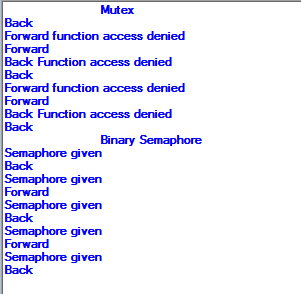
\includegraphics{Binarymutex}
\end{frame}

\begin{frame}
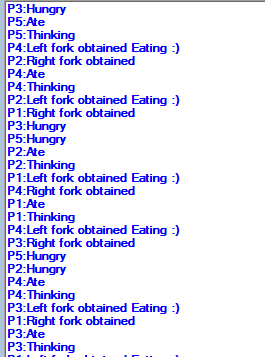
\includegraphics{Dinning}
\end{frame}
\begin{frame}
	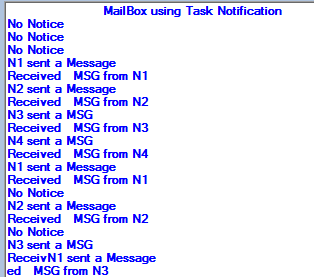
\includegraphics{mbox}
\end{frame}

\begin{frame}
	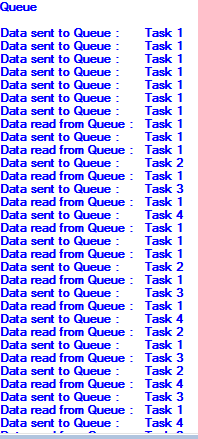
\includegraphics{queue}
\end{frame}

\section{Challenges Faced}
\begin{frame}{Challenges Faced}
    \begin{itemize}
        \item \textbf{Issue} : Porting RTOS into Firebird V and the configurations that needed changes.
        \item Solution : Replace the startup.s file and include various other libraries.
        
        \item Finding Implementation level difference between Binary Semaphore and Mutex.
        
        \item \textbf{Issue} : Loss of Data in Serial Communication.
        \item Solution :
        
        \begin{itemize}
        \item Shortening the string size(temporary solution),
        \item Tried creating a Mutex for accessing the Serial communication Functions.
        \item Trying to solve Using Queues
        \end{itemize}
        
    \end{itemize}
\end{frame}
\section{Future Plans}
\begin{frame}{Future Plans}
    \begin{itemize}
        
        \item Smartphone Interfacing with FireBird V.
        \item Create a mini project that can demonstrate all the learnt concepts together.  
        
    \end{itemize}
\end{frame}

\section{References}
\begin{frame}{References}
    \begin{itemize}
        \item http://www.freertos.org
        \item http://tinymicros.com/
        \item http://www.ocfreaks.com/cat/embedded/lpc2148-tutorials/
        \item http://www.rtos.be/2013/05/mutexes-and-semaphores-two-concepts-for-two-different-use-cases/
    \end{itemize}
\end{frame}

\section{Thank You}
\begin{frame}{Thank You}
    \centering THANK YOU !!!
\end{frame}
\end{document}